\documentclass[11pt,a4paper]{article}

\usepackage[utf8]{inputenc}
\usepackage[ukrainian]{babel}
\usepackage[T2A]{fontenc}
\usepackage{graphicx}
\usepackage{titlesec}
\usepackage{geometry}
\usepackage{xcolor}
\usepackage[colorlinks=true, linkcolor=blue, urlcolor=blue]{hyperref}

\geometry{margin=2.5cm}

\begin{document}

\begin{titlepage}
    \centering

    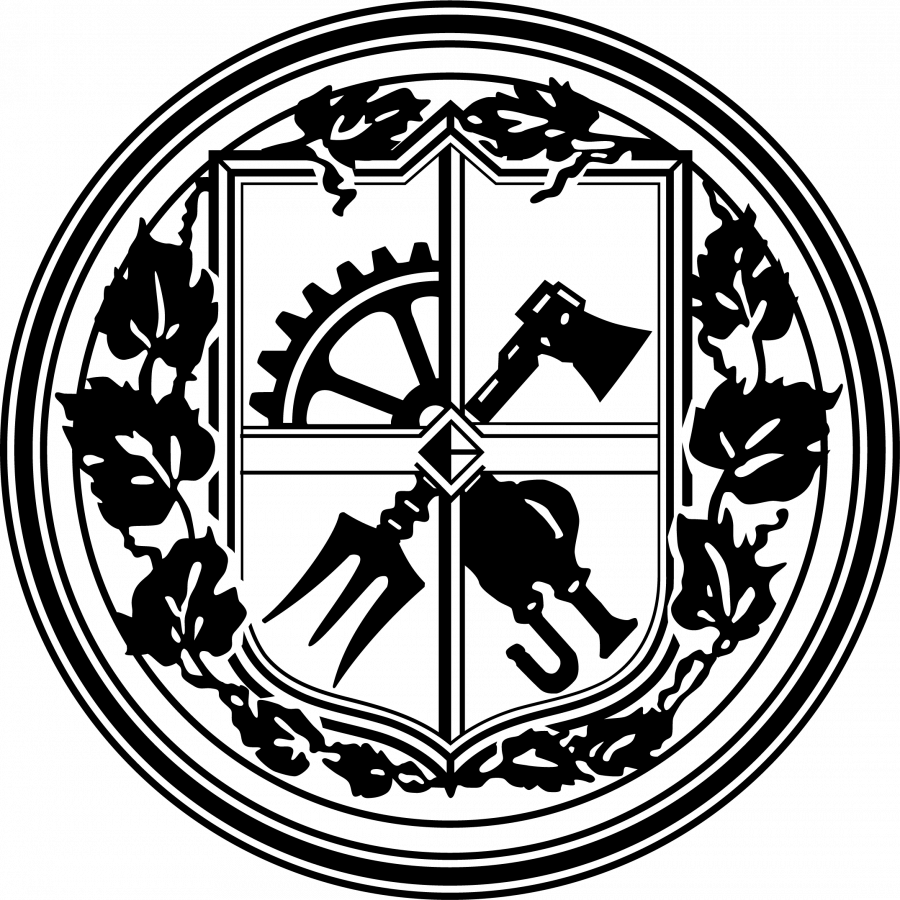
\includegraphics[width=0.6\textwidth]{kpi-big-logo.png}

    \vspace{2cm}

    {\Huge \textbf{НАЦІОНАЛЬНИЙ ТЕХНІЧНИЙ УНІВЕРСИТЕТ УКРАЇНИ «КИЇВСЬКИЙ ПОЛІТИХНІЧНИЙ ІНСТИТУТ ІМ.ІГОРЯ СІКОРСЬКОГО»}}

    \vspace{1.5cm}

    {\Large \textcolor{gray}{Бакалаврська робота}}

    \vspace{2cm}

    {\large
    \textbf{Вивчення економіки США для оцінки коефіцієнту інфляції}\\
    \vspace{0.5cm}
    Жуковін Олександр\\
    }

    \vfill

    {\large \today}

\end{titlepage}

\newpage


\section*{\textbf{Мета}}
\addcontentsline{toc}{section}{Мета}

Створити модель для оцінки та прогнозування вірогідності значної зміни коефіцієнту інфляції США на основі набору поточних
економічних факторів. Модель має визначити "критичні" значення набору економічних показників для того щоб оцінити
вірогідність росту інфляції або дефляції.

\section*{\textbf{Завдання}}
\addcontentsline{toc}{section}{Завданняи}

Для досягнення поставленої мети необхідно виконати наступні завдання:
\begin{enumerate}
    \item Визначити набір економічних показників для побудови моделі;
    \item Проаналізувати історичні дані по інфляції США;
        \begin{itemize}
            \item Відібрати основні історичні періоди значних негативних змін інфляції (висока інфляція або дефляція);
            \item Зібрати дані по основних економічних показниках;
            \item Відібрати періоди з стриятливою інфляцією (інфляція в межах 1-2\%);
            \item Зібрати дані по основних економічних показниках;
        \end{itemize}
    \item Дослідити кореляцію між інфляцією та основними економічними показниками;
    \item Побудувати модель для оцінки та прогнозування вірогідності значної зміни коефіцієнту інфляції США на основі набору поточних економічних факторів;
    \item Провести тести моделі на адекватність та надійність;
    \item Порахувати "точність" моделі;
\end{enumerate}

\section*{\textbf{Об'єкт дослідження}}
\addcontentsline{toc}{section}{Об'єкт дослідження}

Об'єктом дослідження є економіка США, її фінансові ринки, макроекономічні показники та інфляційні процеси.

\section*{\textbf{Предмет дослідження}}
\addcontentsline{toc}{section}{Предмет дослідження}

Для створення моделі необхідні такі аспекти економіки США як:
\begin{itemize}
    \item Макроекономічні показники (ВВП, рівень безробіття, процентні ставки, обсяг експорту та імпорту, обсяг споживання тощо);
    \item Фінансові ринки (показники основних індексів фондових ринків);
    \item Інфляційні процеси (індекс споживчих цін, індекс промислового виробництва тощо);
\end{itemize}

\section*{\textbf{Актуальність дослідження}}
\addcontentsline{toc}{section}{Актуальність дослідження}

Загалому складно переоцінити актуальність інституту грошей, зокрема дослідження інфляції, в будь-який період часу.
Проте, саме в сьогоденні існують прицеденти що вказують на проблему зростання інфляції, зокрема в США. Тому дослідження
цієї проблеми несе в собі окрім пізнавальної, ще й практичну цінність.

\newpage
\noindent Нижче наведені джерела що демонструють проблему інфляції:
\begin{itemize}
    \item International Monetary Fund: \href{https://www.imf.org/en/Publications/WEO/Issues/2025/07/29/world-economic-outlook-update-july-2025}{World Economic Outlook Update: 2025};
    \item Ernst \& Young: \href{https://www.ey.com/en_us/insights/strategy/macroeconomics/us-economic-outlook}{US Economic Outlook September 2025};
    \item S\&P Global: \href{https://www.spglobal.com/ratings/en/regulatory/article/economic-outlook-us-q4-2025-below-trend-growth-persists-amid-a-swirl-of-policy-shifts-s101646549}{Economic Outlook U.S. Q4 2025};
\end{itemize}


\section*{\textbf{Наукова новизна}}
\addcontentsline{toc}{section}{Наукова новизна}

Враховуючи сучасний прогрес у розвитку нейронних мереж в багатьох прикладних сферах та важливість дослідження економічних процесів,
буде актуальним використання сучасних технологій для аналізу економіки. Ця робота дозволить використати існуючі методи дослідження,
об'єднати їх та автоматизувати комплекний аналіз економіки з урахуванням відразу кількох основних факторів.


\newpage


\end{document}
